\section{Symbolic Analysis}
The aim of symbolic analysis is to find the set of non-zero locations (\(\chi\)). 
This can be achieved using the second part of Gilbert-Peierls' algorithm (Algorithm \ref{algo:GP_tri}).
The non-zero elements in column $i$ can be found using the following equations:

\begin{subequations}
    \centering
    \begin{align}
        (b_i \neq 0) &\implies (x_i \neq 0) \\
        (x_j \neq 0) and \exists i(l_{ij} \neq 0) &\implies (x_i \neq 0)
    \end{align}
    \label{eqn:sym:findingX}
\end{subequations}

\begin{figure}[h]
    \centering
    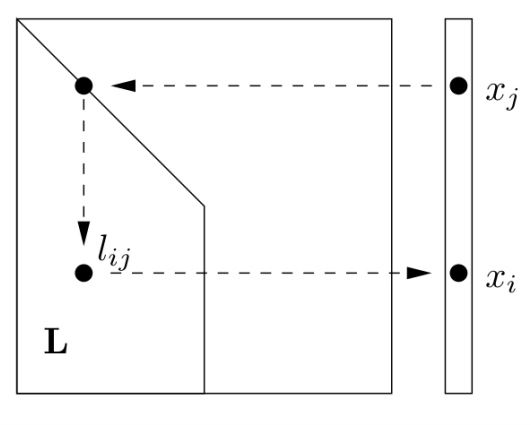
\includegraphics[width = 0.45\textwidth]{./Theory/nnzPattern.JPG}
    \caption{Non-zero pattern in LU decomposition}
    \label{fig:sym:nnzPattern}
\end{figure}

These two implications can be modelled as a traversal of a DAG representing the 
column dependance of the lower triangular section of graph $A$ \cite{Nechma}.
The set ($S$) of non-zero elements in any column ($j$) is given by 
\begin{equation}
    \centering
    s = \bigcup \limits_{x_{ij} \in a_j} Reach(x_{ij})
    \label{eqn:symNZ}
\end{equation}
where $a_j$ is a column vector of matrix $A$ and the $Reach(x)$ is defined as the 
location of non-zero elements in the $x^{th}$ column of the factor matrix which below the diagonal of the matrix. 
The reach of each column then has to be updated as fill ins may have been added to the column of factor matrix.
The location of fill-ins can be found
by removing the non-zero locations in $a_{ij}$ from $S$ as follows:
\begin{equation}
    \centering
    fillIn(j) = reach(j) - \{i|x_{ij}\neq 0\}
    \label{en:fillIns}
\end{equation}
To illustrate the algorithm consider the matrix $A$ shown in the following figure
\ref{fig:sym:example}. The bullets $(\bullet)$ represent non zero entries in the original matrix
and the circles $(\circ)$ represent the location of fill-ins. For example if we look 
at the column zero, it has non-zero elements at row indices 2 and 3. Therfore the $Reach(0) = \{2, 3\}$. It means that
any column with column index greater than 0 having a non-zero element at row index 0
will have non-zero elements at the row indices 2 and 3. Since columns 2 and 4 
satisfy the above condition they have non-zero elements at row indices 2 and 3 in the
factor matrix.

\begin{equation*}
    \begin{split}
        NonZero(Col_2) &= Reach(0, 2, 5) \\
        &= Reach(0) \cup Reach(2) \cup Reach(5) \\
        &= \{0, 2, 3\} \cup \{2, 5\} \cup \{5\} \\
        &= \{0, 2, 3, 5\}
    \end{split}
\end{equation*}

and hence the new reach of column 2 is $\{2, 3, 5\}$ location of fill-ins in column 2 are

\begin{equation*}
    \begin{split}
        fillIns(Col_2) &= Reach(2) - \{0, 2, 5\} \\
        &= \{3\}
    \end{split}
\end{equation*} 

\begin{figure}[h]
    \centering
    \begin{subfigure}[b]{0.5\textwidth}
        \centering
        \begin{tabular}{|c|c|c|c|c|}
        \hline
        \cellcolor{gray!80} $\bullet$   &                               &         $\bullet$            &                               &         $\bullet$     \\ 
        \hline
        \cellcolor{gray!80}             & \cellcolor{gray!80} $\bullet$ &                               &      $\bullet$                &                     \\ 
        \hline
        \cellcolor{gray!80} $\bullet$   & \cellcolor{gray!80}           & \cellcolor{gray!80} $\bullet$ &                               &          $\circ$    \\ 
        \hline
        \cellcolor{gray!80} $\bullet$   & \cellcolor{gray!80} $\bullet$ & \cellcolor{gray!80} $\circ$   & \cellcolor{gray!80} $\bullet$ &         $\circ$           \\ 
        \hline
        \cellcolor{gray!80}             & \cellcolor{gray!80}           & \cellcolor{gray!80} $\bullet$ & \cellcolor{gray!80}           & \cellcolor{gray!80} $\bullet$ \\ 
        \hline
        \end{tabular}
        \caption{Matrix with asymmetric non-zero pattern}
        \label{fig:sym:exampleMat}
    \end{subfigure}%
    \begin{subfigure}[b]{.5\textwidth}
        \centering
        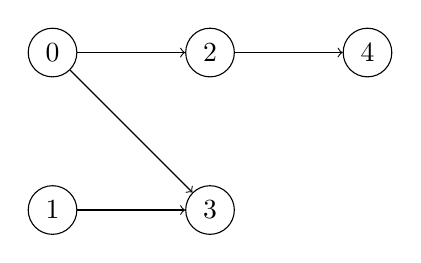
\begin{tikzpicture}
            \node[shape=circle,draw=black] (0) at (0,0) {0};
            \node[shape=circle,draw=black] (1) at (0,-2) {1};
            \node[shape=circle,draw=black] (2) at (2,0) {2};
            \node[shape=circle,draw=black] (3) at (2,-2) {3};
            \node[shape=circle,draw=black] (4) at (4,0) {4};

            \path [->] (0) edge (2);
            \path [->] (2) edge (4);
            \path [->] (0) edge (3);
            \path [->] (1) edge (3);
        \end{tikzpicture}
        \caption{Column dependency graph}
        \label{fig:sym:colDepGraph}
    \end{subfigure}
    \caption{Example of Symbolic Analysis}
    \label{fig:sym:example}
\end{figure}

\section{Generating Computational Flow Graph}

The computational flow graph is a directed acyclic graph of all the operations
which are required to compute the factor matrix. Each node of the graph represents
single arithmetic operation such as MAC and divide. The children nodes of a particular
node represents the elements required to compute the give node and hence the children
must be executed before executing the parent node. A calculation of single element
may require multiple MAC operations and may or may not require divide operation (normalization) depending
on the location of the element in the matrix. For example in the factorization of the example matrix 
(figure \ref{fig:sym:exampleMat})
$U_{3,4} = A_{3,4} - U_{2,4}L_{3,0} - U_{0,4}L_{3_2}$. Since there are multiple 
atomic MAC operations and we can not execute them parallelly, the scheduling has to schedule one ofter the another.
The scheduler can not determine which of the required multiplicands will be ready first using the flow graph.
The task graph must represent all the possibilities for the execution of particular node (figure \ref{fig:sym:example:mac}). This
problem is solved by generating super node for all the AMC operations required for particular element. 
which require more than one. This allows scheduler to determine the operation sequence 
based on the availability for operands.

\begin{figure}
    \centering
    \begin{subfigure}[t]{0.32\textwidth}
        \centering
        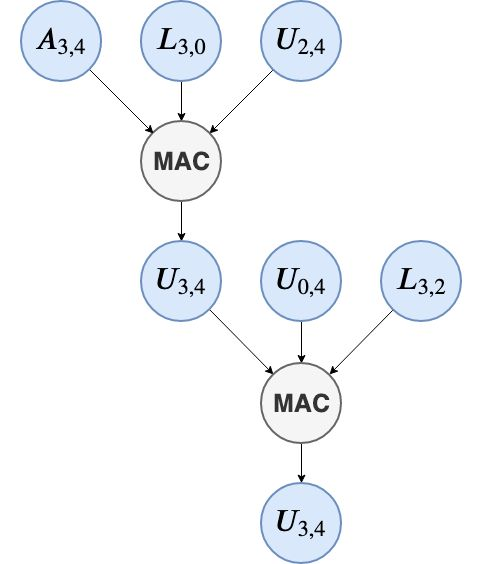
\includegraphics[width = \textwidth]{./Scheduler/macNode1.jpg}
        \caption{Dependency graph for the node $U_{3,4}$}
        \label{fig:sym:example:mac0}
    \end{subfigure}
    \hfill
    \begin{subfigure}[t]{0.32\textwidth}
        \centering
        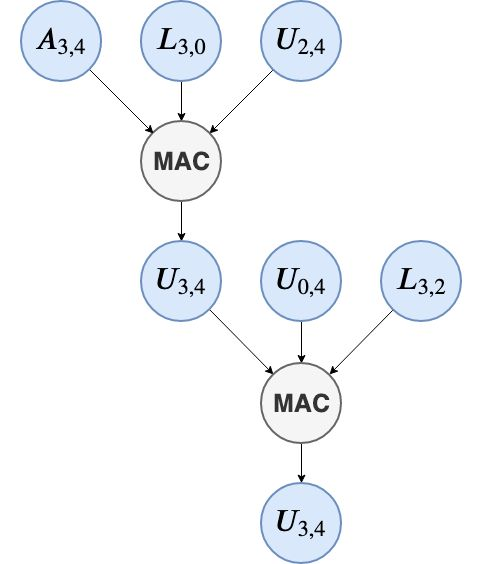
\includegraphics[width = \textwidth]{./Scheduler/macNode1.jpg}
        \caption{Execution option 1}
        \label{fig:sym:example:mac1}
    \end{subfigure}
    \hfill
    \begin{subfigure}[t]{0.32\textwidth}
        \centering
        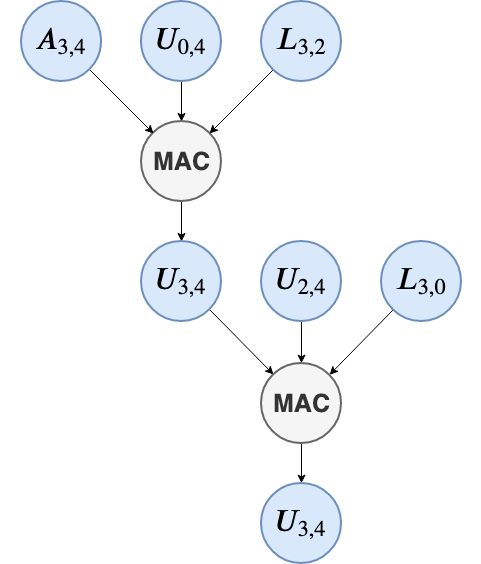
\includegraphics[width = \textwidth]{./Scheduler/macNode2.jpg}
        \caption{Execution option 2}
        \label{fig:sym:example:mac2}
    \end{subfigure}
    \caption{Example showing multiple possible computation flows for the single MAC element}
    \label{fig:sym:example:mac}
\end{figure}


The computation flow can be generated in symbolic analysis itself without much overload as we already know 
the positions of non-zero elements and the elements which are responsible for making them non-zero . 
The figure \ref{fig:sym:flowGraph} shows the 
computational flow graph for the example matrix shown in figure \ref{fig:sym:exampleMat}.

\begin{figure}
    \centering
    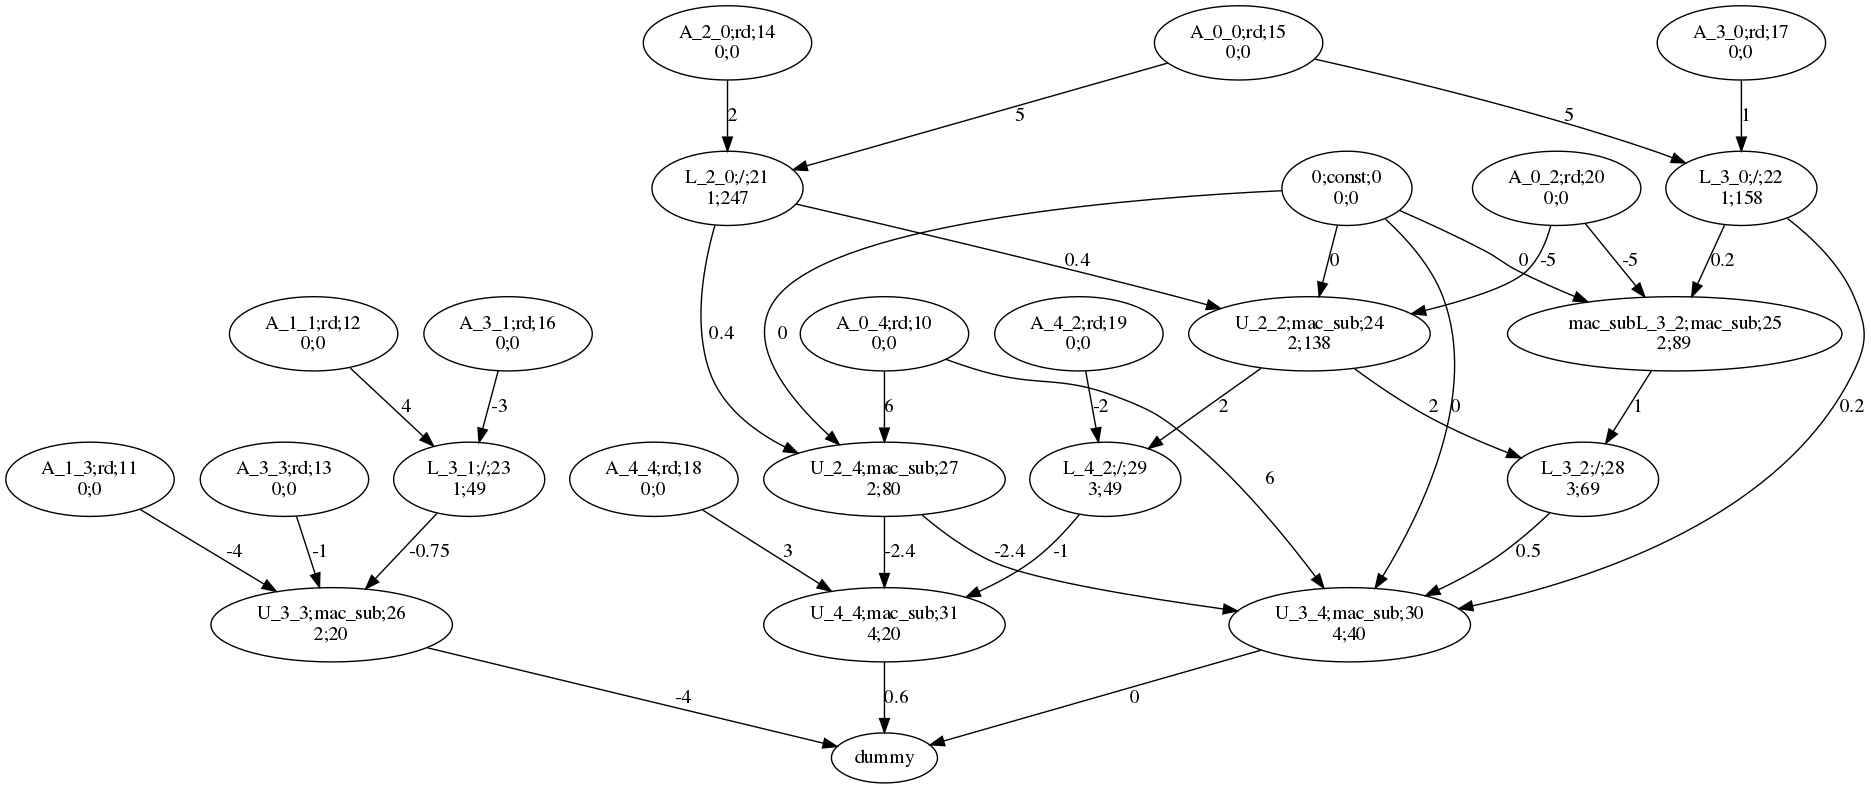
\includegraphics[width = \textwidth]{./Scheduler/exeTree.png}
    \caption{Computational flow graph for example matrix shown in figure \ref{fig:sym:exampleMat}}
    \label{fig:sym:flowGraph}
\end{figure}

